\section{Post-Quantum Cryptography Preview}

\subsection{Ancaman Quantum Computing terhadap Kriptografi Modern}

Komputer quantum menimbulkan ancaman eksistensial terhadap kriptografi modern yang kita pelajari sejauh ini \cite{shor1997}. Algoritma quantum dapat memecahkan masalah matematis yang menjadi fondasi keamanan cipher klasik.

\textbf{Algoritma Quantum yang Berbahaya}:
\begin{itemize}
  \item \textbf{Shor's Algorithm (1994)}: Memfaktorkan bilangan besar dan menyelesaikan discrete logarithm dalam waktu polinomial
  \item \textbf{Grover's Algorithm (1996)}: Mencari dalam database tidak terstruktur dengan kompleksitas $O(\sqrt{N})$
\end{itemize}

\begin{table}[htbp]
  \centering
  \small
  \begin{tabular}{lcc}
    \toprule
    Algoritma & Komputer Klasik & Komputer Quantum \\
    \midrule
    Faktorisasi RSA-2048 & $2^{112}$ operasi & Beberapa menit \\
    Discrete Logarithm ECC-256 & $2^{128}$ operasi & Beberapa menit \\
    Brute Force AES-128 & $2^{127}$ operasi & $2^{64}$ operasi \\
    \bottomrule
  \end{tabular}
  \caption{Perbandingan kompleksitas komputasi klasik vs quantum.}
\end{table}

\subsection{Kategori Post-Quantum Cryptography}

NIST mengidentifikasi lima kategori utama post-quantum cryptography \cite{nist2016}:

\begin{enumerate}
  \item \textbf{Lattice-based Cryptography}: Berdasarkan kesulitan Shortest Vector Problem (SVP)
  \item \textbf{Hash-based Signatures}: Berdasarkan fungsi hash one-way
  \item \textbf{Code-based Cryptography}: Berdasarkan kesulitan decoding error-correcting codes
  \item \textbf{Multivariate Cryptography}: Berdasarkan kesulitan menyelesaikan sistem persamaan kuadrat
  \item \textbf{Isogeny-based Cryptography}: Berdasarkan kesulitan isogeny antar kurva eliptik
\end{enumerate}

\subsection{Lattice-based Cryptography}

Lattice-based cryptography adalah kandidat paling menjanjikan untuk post-quantum cryptography \cite{regev2009}. Keamanannya didasarkan pada kesulitan masalah lattice seperti Shortest Vector Problem (SVP) dan Learning With Errors (LWE).

\subsubsection{Learning With Errors (LWE)}

LWE problem: Diberikan matriks acak $A$ dan vektor $\mathbf{b} = A\mathbf{s} + \mathbf{e}$, temukan $\mathbf{s}$ dimana $\mathbf{e}$ adalah vektor error kecil.

\begin{lstlisting}[style=cstyle, caption={LWE Key Exchange}]
#include <stdint.h>
#include <stdlib.h>

#define N 512  // Dimension
#define Q 3329 // Modulus

typedef struct {
    int16_t a[N];
    int16_t b;
} LWESample;

// Generate LWE sample
void generate_lwe_sample(int16_t secret[N], LWESample *sample) {
    // Random vector a
    for (int i = 0; i < N; i++) {
        sample->a[i] = random_int(0, Q-1);
    }
    
    // Compute b = a*s + e (mod q)
    int32_t dot_product = 0;
    for (int i = 0; i < N; i++) {
        dot_product += sample->a[i] * secret[i];
    }
    
    // Add small error
    int16_t error = random_gaussian(0, 3); // Small Gaussian error
    
    sample->b = (dot_product + error) % Q;
}

// LWE key exchange
void lwe_key_exchange() {
    int16_t alice_secret[N], bob_secret[N];
    LWESample alice_sample, bob_sample;
    
    // Generate secrets
    for (int i = 0; i < N; i++) {
        alice_secret[i] = random_int(0, Q-1);
        bob_secret[i] = random_int(0, Q-1);
    }
    
    // Alice generates sample and sends to Bob
    generate_lwe_sample(alice_secret, &alice_sample);
    
    // Bob computes his contribution
    int32_t bob_contribution = 0;
    for (int i = 0; i < N; i++) {
        bob_contribution += alice_sample.a[i] * bob_secret[i];
    }
    
    // Alice computes shared secret
    int32_t alice_shared = 0;
    for (int i = 0; i < N; i++) {
        alice_shared += alice_sample.a[i] * bob_secret[i];
    }
    
    // Both should have approximately the same shared secret
    printf("Alice shared: %d\n", alice_shared % Q);
    printf("Bob shared: %d\n", bob_contribution % Q);
}
\end{lstlisting}

\subsubsection{Kyber - Lattice-based KEM}

Kyber adalah finalist NIST PQC competition untuk Key Encapsulation\\ Mechanism (KEM) \cite{bos2018}.

\begin{lstlisting}[style=cstyle, caption={Kyber KEM Simplified}]
typedef struct {
    uint16_t poly[256];
} Polynomial;

// NTT (Number Theoretic Transform) for polynomial multiplication
void ntt(Polynomial *poly) {
    for (int len = 2; len <= 256; len *= 2) {
        for (int i = 0; i < 256; i += len) {
            for (int j = 0; j < len/2; j++) {
                // Butterfly operation
                uint16_t u = poly[i + j];
                uint16_t v = poly[i + j + len/2] * zeta[len/2 + j];
                
                poly[i + j] = (u + v) % Q;
                poly[i + j + len/2] = (u - v + Q) % Q;
            }
        }
    }
}

// Kyber key generation
void kyber_keygen(Polynomial *pk, Polynomial *sk) {
    // Generate secret polynomial
    for (int i = 0; i < 256; i++) {
        sk->poly[i] = random_centered_binomial(2);
    }
    
    // Generate public polynomial
    Polynomial a, e;
    for (int i = 0; i < 256; i++) {
        a.poly[i] = random_uniform(Q);
        e.poly[i] = random_centered_binomial(2);
    }
    
    // pk = a * sk + e
    polynomial_multiply(&a, sk, pk);
    polynomial_add(pk, &e, pk);
}

// Kyber encapsulation
void kyber_encapsulate(Polynomial *pk, uint8_t *ciphertext, uint8_t *shared_secret) {
    Polynomial m, r, e1, e2;
    
    // Generate random message and blinder
    for (int i = 0; i < 256; i++) {
        m.poly[i] = random_centered_binomial(1);
        r.poly[i] = random_centered_binomial(2);
    }
    
    // Compute ciphertext components
    Polynomial u, v;
    polynomial_multiply(pk, &r, &u);
    
    for (int i = 0; i < 256; i++) {
        e1.poly[i] = random_centered_binomial(2);
        e2.poly[i] = random_centered_binomial(2);
    }
    
    polynomial_add(&u, &e1, &u);
    polynomial_multiply(&m, &r, &v);
    polynomial_add(&v, &e2, &v);
    
    // Encode and compress
    encode_polynomial(&u, ciphertext);
    encode_polynomial(&v, ciphertext + 256);
    
    // Derive shared secret
    kdf(m.poly, 256, shared_secret, 32);
}
\end{lstlisting}

\subsection{Hash-based Signatures}

Hash-based signatures menggunakan fungsi hash one-way sebagai satu-satunya asumsi keamanan \cite{merkle1979}. Lamport signatures adalah skema dasar, sementara Merkle signatures mengoptimalkan untuk multiple signatures.

\subsubsection{Lamport One-Time Signatures}

\begin{lstlisting}[style=cstyle, caption={Lamport One-Time Signature}]
#include <stdint.h>
#include <openssl/sha.h>

#define HASH_SIZE 32
#define KEY_SIZE 256

typedef struct {
    uint8_t sk_0[KEY_SIZE][HASH_SIZE]; // Private key for 0 bits
    uint8_t sk_1[KEY_SIZE][HASH_SIZE]; // Private key for 1 bits
    uint8_t pk_0[KEY_SIZE][HASH_SIZE]; // Public key for 0 bits
    uint8_t pk_1[KEY_SIZE][HASH_SIZE]; // Public key for 1 bits
} LamportKeyPair;

// Generate Lamport key pair
void lamport_keygen(LamportKeyPair *keys) {
    for (int i = 0; i < KEY_SIZE; i++) {
        // Generate private keys
        random_bytes(keys->sk_0[i], HASH_SIZE);
        random_bytes(keys->sk_1[i], HASH_SIZE);
        
        // Compute public keys by hashing
        SHA256(keys->sk_0[i], HASH_SIZE, keys->pk_0[i]);
        SHA256(keys->sk_1[i], HASH_SIZE, keys->pk_1[i]);
    }
}

// Sign message
void lamport_sign(uint8_t *message, size_t msg_len, 
                  LamportKeyPair *keys, uint8_t *signature) {
    uint8_t hash[HASH_SIZE];
    SHA256(message, msg_len, hash);
    
    for (int i = 0; i < KEY_SIZE; i++) {
        int bit = (hash[i/8] >> (i % 8)) & 1;
        
        if (bit == 0) {
            memcpy(signature + i * HASH_SIZE, keys->sk_0[i], HASH_SIZE);
        } else {
            memcpy(signature + i * HASH_SIZE, keys->sk_1[i], HASH_SIZE);
        }
    }
}

// Verify signature
int lamport_verify(uint8_t *message, size_t msg_len, 
                   uint8_t *signature, LamportKeyPair *keys) {
    uint8_t hash[HASH_SIZE];
    SHA256(message, msg_len, hash);
    
    for (int i = 0; i < KEY_SIZE; i++) {
        int bit = (hash[i/8] >> (i % 8)) & 1;
        
        uint8_t computed_hash[HASH_SIZE];
        SHA256(signature + i * HASH_SIZE, HASH_SIZE, computed_hash);
        
        if (bit == 0) {
            if (memcmp(computed_hash, keys->pk_0[i], HASH_SIZE) != 0) {
                return 0; // Verification failed
            }
        } else {
            if (memcmp(computed_hash, keys->pk_1[i], HASH_SIZE) != 0) {
                return 0; // Verification failed
            }
        }
    }
    
    return 1; // Verification successful
}
\end{lstlisting}

\subsubsection{XMSS - Extended Merkle Signature Scheme}

XMSS adalah stateful hash-based signature scheme yang efisien untuk multiple signatures \cite{bucha2011}.

\begin{lstlisting}[style=cstyle, caption={XMSS Tree Building}]
#define TREE_HEIGHT 10
#define LEAF_COUNT (1 << TREE_HEIGHT)

typedef struct TreeNode {
    uint8_t hash[HASH_SIZE];
    struct TreeNode *left;
    struct TreeNode *right;
} TreeNode;

// Build Merkle tree
TreeNode* build_merkle_tree(uint8_t *leaves, int leaf_count) {
    TreeNode *nodes[LEAF_COUNT * 2 - 1];
    
    // Create leaf nodes
    for (int i = 0; i < leaf_count; i++) {
        nodes[leaf_count - 1 + i] = malloc(sizeof(TreeNode));
        memcpy(nodes[leaf_count - 1 + i]->hash, leaves + i * HASH_SIZE, HASH_SIZE);
    }
    
    // Build internal nodes
    for (int i = leaf_count - 2; i >= 0; i--) {
        nodes[i] = malloc(sizeof(TreeNode));
        nodes[i]->left = nodes[2 * i + 1];
        nodes[i]->right = nodes[2 * i + 2];
        
        // Hash children
        uint8_t combined[HASH_SIZE * 2];
        memcpy(combined, nodes[i]->left->hash, HASH_SIZE);
        memcpy(combined + HASH_SIZE, nodes[i]->right->hash, HASH_SIZE);
        
        SHA256(combined, HASH_SIZE * 2, nodes[i]->hash);
    }
    
    return nodes[0]; // Return root
}

// Generate XMSS authentication path
void generate_auth_path(TreeNode *root, int leaf_index, 
                      uint8_t auth_path[TREE_HEIGHT][HASH_SIZE]) {
    // Traverse tree to find authentication path
    TreeNode *current = root;
    int path_index = 0;
    
    for (int level = 0; level < TREE_HEIGHT; level++) {
        int bit = (leaf_index >> (TREE_HEIGHT - 1 - level)) & 1;
        
        if (bit == 0) {
            // Take right sibling
            memcpy(auth_path[path_index++], current->right->hash, HASH_SIZE);
            current = current->left;
        } else {
            // Take left sibling
            memcpy(auth_path[path_index++], current->left->hash, HASH_SIZE);
            current = current->right;
        }
    }
}
\end{lstlisting}

\subsection{Code-based Cryptography}

Code-based cryptography didasarkan pada kesulitan decoding general linear codes \cite{mceliece1978}. McEliece adalah skema enkripsi tertua yang resisten terhadap serangan quantum.

\subsubsection{McEliece Cryptosystem}

\begin{lstlisting}[style=cstyle, caption={McEliece Key Generation}]
#define N 2048  // Code length
#define K 1024  // Message length
#define T 41    // Error capability

typedef struct {
    uint8_t G[K][N];  // Generator matrix
    uint8_t P[N][N];  // Permutation matrix
    uint8_t S[K][K];  // Invertible matrix
} McEliecePrivateKey;

typedef struct {
    uint8_t G_pub[K][N];  // Public generator matrix
    uint8_t t;            // Error capability
} McEliecePublicKey;

// Generate McEliece key pair
void mceliece_keygen(McEliecePrivateKey *priv, McEliecePublicKey *pub) {
    // Generate random invertible matrix S
    generate_random_invertible_matrix(priv->S, K);
    
    // Generate random permutation matrix P
    generate_random_permutation_matrix(priv->P, N);
    
    // Generate Goppa code generator matrix G
    generate_goppa_generator_matrix(priv->G, K, N, T);
    
    // Compute public key: G_pub = S * G * P
    matrix_multiply(priv->S, priv->G, temp_matrix, K, K, N);
    matrix_multiply(temp_matrix, priv->P, pub->G_pub, K, N, N);
    
    pub->t = T;
}

// McEliece encryption
void mceliece_encrypt(uint8_t *message, McEliecePublicKey *pub, 
                     uint8_t *ciphertext) {
    uint8_t m[K], c[N], e[N];
    
    // Pad message to K bits
    memcpy(m, message, K);
    
    // Compute c = m * G_pub
    matrix_vector_multiply(pub->G_pub, m, c, K, N);
    
    // Add random error vector e with weight t
    generate_error_vector(e, N, pub->t);
    vector_add(c, e, ciphertext, N);
}

// McEliece decryption
void mceliece_decrypt(uint8_t *ciphertext, McEliecePrivateKey *priv, 
                     uint8_t *message) {
    uint8_t c[N], m[K];
    
    // Remove permutation: c' = c * P^(-1)
    uint8_t P_inv[N][N];
    matrix_inverse(priv->P, P_inv, N);
    matrix_vector_multiply(P_inv, ciphertext, c, N, N);
    
    // Decode using Goppa code decoder
    goppa_decode(c, priv->G, m, K, N, T);
    
    // Remove S: message = m * S^(-1)
    uint8_t S_inv[K][K];
    matrix_inverse(priv->S, S_inv, K);
    matrix_vector_multiply(S_inv, m, message, K, K);
}
\end{lstlisting}

\subsection{Timeline Quantum Migration}

\textbf{Timeline yang Direkomendasikan}:
\begin{itemize}
  \item \textbf{2024-2026}: Evaluasi dan testing algoritma PQC
  \item \textbf{2026-2030}: Migrasi gradual ke hybrid systems
  \item \textbf{2030+}: Depreciation RSA/ECC untuk aplikasi baru
\end{itemize}

\begin{figure}[htbp]
  \centering
  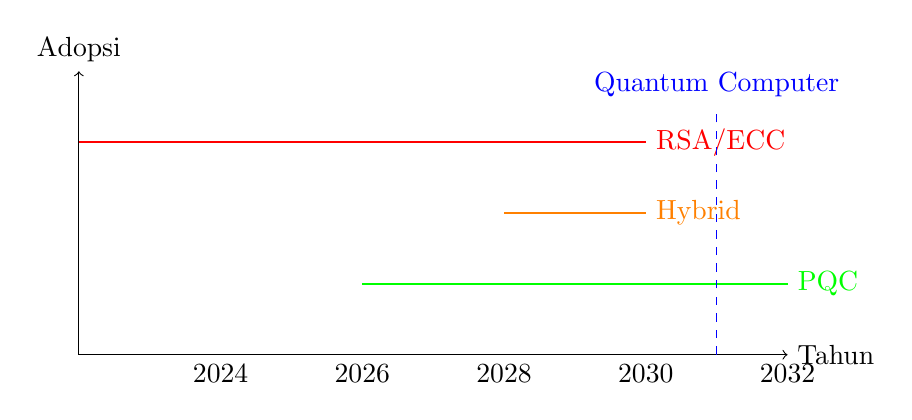
\begin{tikzpicture}[scale=0.9]
    \draw[->] (0,0) -- (10,0) node[right] {Tahun};
    \draw[->] (0,0) -- (0,4) node[above] {Adopsi};
    
    % Classical cryptography
    \draw[thick, red] (0,3) -- (8,3) node[right] {RSA/ECC};
    
    % Hybrid period
    \draw[thick, orange] (6,2) -- (8,2) node[right] {Hybrid};
    
    % Post-quantum
    \draw[thick, green] (4,1) -- (10,1) node[right] {PQC};
    
    % Quantum threat
    \draw[dashed, blue] (9,0) -- (9,3.5) node[above] {Quantum Computer};
    
    % Labels
    \node[below] at (2,0) {2024};
    \node[below] at (4,0) {2026};
    \node[below] at (6,0) {2028};
    \node[below] at (8,0) {2030};
    \node[below] at (10,0) {2032};
  \end{tikzpicture}
  \caption{Timeline migrasi ke post-quantum cryptography.}
\end{figure}

\subsection{Implementasi Praktis}

\textbf{Library Post-Quantum}:
\begin{itemize}
  \item \textbf{PQCrypto}: Implementasi referensi NIST PQC finalists
  \item \textbf{liboqs}: Open Quantum Safe library
  \item \textbf{OpenSSL 3.0+}: Dukungan PQC eksperimental
  \item \textbf{Bouncy Castle}: Implementasi Java untuk PQC
\end{itemize}

\begin{lstlisting}[style=cstyle, caption={Hybrid TLS 1.3 with PQC}]
// Hybrid key exchange: ECDHE + Kyber
int hybrid_key_exchange() {
    uint8_t ecdhe_shared[32], kyber_shared[32];
    uint8_t hybrid_shared[64];
    
    // Perform ECDHE key exchange
    ecdhe_key_exchange(ecdhe_shared);
    
    // Perform Kyber key exchange
    kyber_key_exchange(kyber_shared);
    
    // Combine shared secrets
    memcpy(hybrid_shared, ecdhe_shared, 32);
    memcpy(hybrid_shared + 32, kyber_shared, 32);
    
    // Derive final key
    uint8_t final_key[32];
    hkdf_extract(NULL, hybrid_shared, 64, final_key);
    
    return 0;
}
\end{lstlisting}

\subsection{Kesimpulan dan Persiapan}

Post-quantum cryptography bukan lagi teori akademis—ini adalah kebutuhan praktis yang mendesak. Organisasi harus:

\begin{enumerate}
  \item \textbf{Inventory}: Identifikasi sistem yang menggunakan kriptografi vulnerable
  \item \textbf{Plan}: Buat roadmap migrasi ke PQC
  \item \textbf{Test}: Evaluasi performance dan compatibility
  \item \textbf{Implement}: Mulai migrasi gradual dengan hybrid systems
\end{enumerate}

\begin{catatan}
Implementasi post-quantum cryptography dari contoh di atas adalah untuk tujuan edukasi. Untuk produksi, gunakan library yang telah melalui standardization process seperti NIST PQC finalists.
\end{catatan}
